% Options for packages loaded elsewhere
\PassOptionsToPackage{unicode}{hyperref}
\PassOptionsToPackage{hyphens}{url}
\PassOptionsToPackage{dvipsnames,svgnames,x11names}{xcolor}
%
\documentclass[
  10pt,
  ignorenonframetext,
  aspectratio=169]{beamer}
\usepackage{pgfpages}
\setbeamertemplate{caption}[numbered]
\setbeamertemplate{caption label separator}{: }
\setbeamercolor{caption name}{fg=normal text.fg}
\beamertemplatenavigationsymbolsempty
% Prevent slide breaks in the middle of a paragraph
\widowpenalties 1 10000
\raggedbottom
\setbeamertemplate{part page}{
  \centering
  \begin{beamercolorbox}[sep=16pt,center]{part title}
    \usebeamerfont{part title}\insertpart\par
  \end{beamercolorbox}
}
\setbeamertemplate{section page}{
  \centering
  \begin{beamercolorbox}[sep=12pt,center]{part title}
    \usebeamerfont{section title}\insertsection\par
  \end{beamercolorbox}
}
\setbeamertemplate{subsection page}{
  \centering
  \begin{beamercolorbox}[sep=8pt,center]{part title}
    \usebeamerfont{subsection title}\insertsubsection\par
  \end{beamercolorbox}
}
\AtBeginPart{
  \frame{\partpage}
}
\AtBeginSection{
  \ifbibliography
  \else
    \frame{\sectionpage}
  \fi
}
\AtBeginSubsection{
  \frame{\subsectionpage}
}
\usepackage{amsmath,amssymb}
\usepackage{lmodern}
\usepackage{iftex}
\ifPDFTeX
  \usepackage[T1]{fontenc}
  \usepackage[utf8]{inputenc}
  \usepackage{textcomp} % provide euro and other symbols
\else % if luatex or xetex
  \usepackage{unicode-math}
  \defaultfontfeatures{Scale=MatchLowercase}
  \defaultfontfeatures[\rmfamily]{Ligatures=TeX,Scale=1}
\fi
\usetheme[]{Singapore}
% Use upquote if available, for straight quotes in verbatim environments
\IfFileExists{upquote.sty}{\usepackage{upquote}}{}
\IfFileExists{microtype.sty}{% use microtype if available
  \usepackage[]{microtype}
  \UseMicrotypeSet[protrusion]{basicmath} % disable protrusion for tt fonts
}{}
\makeatletter
\@ifundefined{KOMAClassName}{% if non-KOMA class
  \IfFileExists{parskip.sty}{%
    \usepackage{parskip}
  }{% else
    \setlength{\parindent}{0pt}
    \setlength{\parskip}{6pt plus 2pt minus 1pt}}
}{% if KOMA class
  \KOMAoptions{parskip=half}}
\makeatother
\usepackage{xcolor}
\newif\ifbibliography
\usepackage{color}
\usepackage{fancyvrb}
\newcommand{\VerbBar}{|}
\newcommand{\VERB}{\Verb[commandchars=\\\{\}]}
\DefineVerbatimEnvironment{Highlighting}{Verbatim}{commandchars=\\\{\}}
% Add ',fontsize=\small' for more characters per line
\usepackage{framed}
\definecolor{shadecolor}{RGB}{48,48,48}
\newenvironment{Shaded}{\begin{snugshade}}{\end{snugshade}}
\newcommand{\AlertTok}[1]{\textcolor[rgb]{1.00,0.81,0.69}{#1}}
\newcommand{\AnnotationTok}[1]{\textcolor[rgb]{0.50,0.62,0.50}{\textbf{#1}}}
\newcommand{\AttributeTok}[1]{\textcolor[rgb]{0.80,0.80,0.80}{#1}}
\newcommand{\BaseNTok}[1]{\textcolor[rgb]{0.86,0.64,0.64}{#1}}
\newcommand{\BuiltInTok}[1]{\textcolor[rgb]{0.80,0.80,0.80}{#1}}
\newcommand{\CharTok}[1]{\textcolor[rgb]{0.86,0.64,0.64}{#1}}
\newcommand{\CommentTok}[1]{\textcolor[rgb]{0.50,0.62,0.50}{#1}}
\newcommand{\CommentVarTok}[1]{\textcolor[rgb]{0.50,0.62,0.50}{\textbf{#1}}}
\newcommand{\ConstantTok}[1]{\textcolor[rgb]{0.86,0.64,0.64}{\textbf{#1}}}
\newcommand{\ControlFlowTok}[1]{\textcolor[rgb]{0.94,0.87,0.69}{#1}}
\newcommand{\DataTypeTok}[1]{\textcolor[rgb]{0.87,0.87,0.75}{#1}}
\newcommand{\DecValTok}[1]{\textcolor[rgb]{0.86,0.86,0.80}{#1}}
\newcommand{\DocumentationTok}[1]{\textcolor[rgb]{0.50,0.62,0.50}{#1}}
\newcommand{\ErrorTok}[1]{\textcolor[rgb]{0.76,0.75,0.62}{#1}}
\newcommand{\ExtensionTok}[1]{\textcolor[rgb]{0.80,0.80,0.80}{#1}}
\newcommand{\FloatTok}[1]{\textcolor[rgb]{0.75,0.75,0.82}{#1}}
\newcommand{\FunctionTok}[1]{\textcolor[rgb]{0.94,0.94,0.56}{#1}}
\newcommand{\ImportTok}[1]{\textcolor[rgb]{0.80,0.80,0.80}{#1}}
\newcommand{\InformationTok}[1]{\textcolor[rgb]{0.50,0.62,0.50}{\textbf{#1}}}
\newcommand{\KeywordTok}[1]{\textcolor[rgb]{0.94,0.87,0.69}{#1}}
\newcommand{\NormalTok}[1]{\textcolor[rgb]{0.80,0.80,0.80}{#1}}
\newcommand{\OperatorTok}[1]{\textcolor[rgb]{0.94,0.94,0.82}{#1}}
\newcommand{\OtherTok}[1]{\textcolor[rgb]{0.94,0.94,0.56}{#1}}
\newcommand{\PreprocessorTok}[1]{\textcolor[rgb]{1.00,0.81,0.69}{\textbf{#1}}}
\newcommand{\RegionMarkerTok}[1]{\textcolor[rgb]{0.80,0.80,0.80}{#1}}
\newcommand{\SpecialCharTok}[1]{\textcolor[rgb]{0.86,0.64,0.64}{#1}}
\newcommand{\SpecialStringTok}[1]{\textcolor[rgb]{0.80,0.58,0.58}{#1}}
\newcommand{\StringTok}[1]{\textcolor[rgb]{0.80,0.58,0.58}{#1}}
\newcommand{\VariableTok}[1]{\textcolor[rgb]{0.80,0.80,0.80}{#1}}
\newcommand{\VerbatimStringTok}[1]{\textcolor[rgb]{0.80,0.58,0.58}{#1}}
\newcommand{\WarningTok}[1]{\textcolor[rgb]{0.50,0.62,0.50}{\textbf{#1}}}
\usepackage{graphicx}
\makeatletter
\def\maxwidth{\ifdim\Gin@nat@width>\linewidth\linewidth\else\Gin@nat@width\fi}
\def\maxheight{\ifdim\Gin@nat@height>\textheight\textheight\else\Gin@nat@height\fi}
\makeatother
% Scale images if necessary, so that they will not overflow the page
% margins by default, and it is still possible to overwrite the defaults
% using explicit options in \includegraphics[width, height, ...]{}
\setkeys{Gin}{width=\maxwidth,height=\maxheight,keepaspectratio}
% Set default figure placement to htbp
\makeatletter
\def\fps@figure{htbp}
\makeatother
\setlength{\emergencystretch}{3em} % prevent overfull lines
\providecommand{\tightlist}{%
  \setlength{\itemsep}{0pt}\setlength{\parskip}{0pt}}
\setcounter{secnumdepth}{-\maxdimen} % remove section numbering
\newenvironment{cols}[1][]{}{}

\newenvironment{col}[1]{\begin{minipage}{#1}\ignorespaces}{%
\end{minipage}
\ifhmode\unskip\fi
\aftergroup\useignorespacesandallpars}

\def\useignorespacesandallpars#1\ignorespaces\fi{%
#1\fi\ignorespacesandallpars}

\makeatletter
\def\ignorespacesandallpars{%
  \@ifnextchar\par
    {\expandafter\ignorespacesandallpars\@gobble}%
    {}%
}
\makeatother
\ifLuaTeX
  \usepackage{selnolig}  % disable illegal ligatures
\fi
\usepackage[]{natbib}
\bibliographystyle{plainnat}
\IfFileExists{bookmark.sty}{\usepackage{bookmark}}{\usepackage{hyperref}}
\IfFileExists{xurl.sty}{\usepackage{xurl}}{} % add URL line breaks if available
\urlstyle{same} % disable monospaced font for URLs
\hypersetup{
  pdftitle={Fancy NLP},
  pdfauthor={Max Callaghan},
  colorlinks=true,
  linkcolor={Maroon},
  filecolor={Maroon},
  citecolor={Blue},
  urlcolor={blue},
  pdfcreator={LaTeX via pandoc}}

\title{Fancy NLP}
\author{Max Callaghan}
\date{2022-11-23}

\begin{document}
\frame{\titlepage}

\hypertarget{introduction-and-objectives}{%
\section{Introduction and
Objectives}\label{introduction-and-objectives}}

\begin{frame}{Assignment 2}
\protect\hypertarget{assignment-2}{}
Thanks to all who submitted assignment 2. You can expect your grades by
the end of this week week.
\end{frame}

\begin{frame}{Fancy NLP}
\protect\hypertarget{fancy-nlp}{}
Today we arrive at the promised ``fancy NLP''. We'll look at

\begin{enumerate}
  \item<1->\textbf{Transformers} and BERT-based models for machine learning with texts
  \item<2->\textbf{Spacy}: which is a ``swiss-army knife'' for doing various tasks with texts
\end{enumerate}

\only<3->{We are working in python because that is what most of the machine learning and CS people use, and that is where these resources are available}

\only<4->{-> For those new to python you should become slightly more familiar with how we run code in notebooks, what a "package" is, and what the code looks like.}
\end{frame}

\hypertarget{bert}{%
\section{BERT}\label{bert}}

\begin{frame}{BERT}
\protect\hypertarget{bert-1}{}
\begin{cols}

\begin{col}{0.4\textwidth}

\begin{itemize}
  \item<1->BERT - (Bidirectional Encoder Representations from Transformers) is a \textbf{language representation model} which changed how we do NLP.
  
  \item<2->BERT is \textbf{pre-trained} (on a masked language model task cf. WordVectors and a next sentence prediction task) on huge text corpora.
  
  \item<3->It can be \textbf{fine-tuned} on a multitude of different tasks using new data.
  
  \item<4->A fine-tuned BERT model offered a step-change increase in performance.
\end{itemize}

\end{col}

\begin{col}{0.05\textwidth}
~

\end{col}

\begin{col}{0.55\textwidth}

\begin{figure}
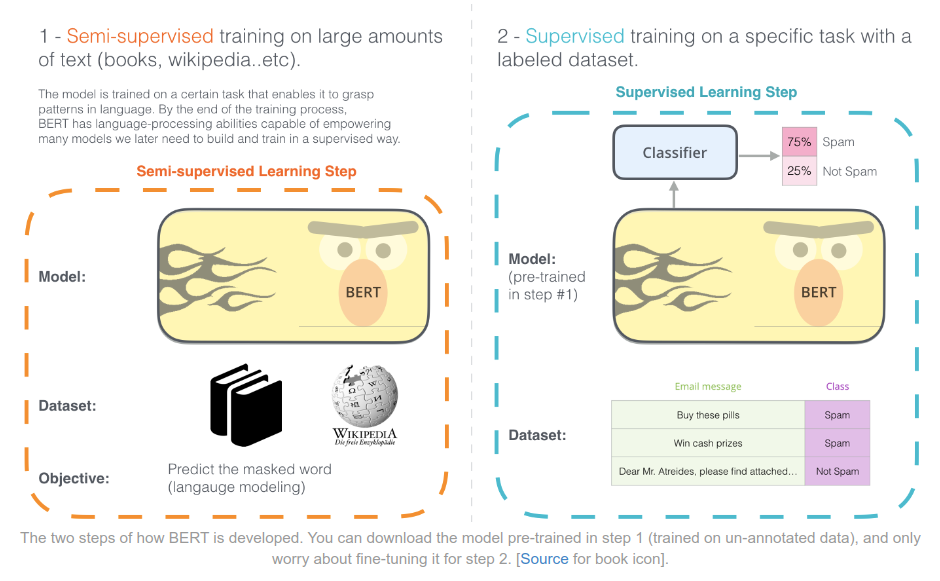
\includegraphics[width=\linewidth]{images/il-bert.png}
\end{figure}

\end{col}

\end{cols}
\end{frame}

\begin{frame}{What's new with BERT}
\protect\hypertarget{whats-new-with-bert}{}
With BERT, the vector representation for each token is \emph{dependent
on its context} (using self-attention).

So, the representation of ``cooler'' will be different in the two
sentences:

\begin{itemize}
\tightlist
\item
  Thursday will see \textbf{cooler} temperatures in the South-East, as a
  cold front moves in'\,'
\item
  The new remake of the film is way \textbf{cooler} than the original.
\end{itemize}

This takes us far beyond bag-of-words. BERT has learnt representations
of texts that are not reliant on such unrealistic assumptions.
\end{frame}

\begin{frame}{What's wrong with BERT}
\protect\hypertarget{whats-wrong-with-bert}{}
However, BERT, and large language models in general have some drawbacks
(see \href{https://dl.acm.org/doi/10.1145/3442188.3445922}{Stochastic
Parrots} among others 
\includegraphics[height=0.5cm]{images/parrot.png}:

\begin{itemize}
  \item<1->Fine-tuning BERT requires more resources
  \item<2->Understanding results and where they come from is harder
  \item<3->Training these models requires enormous resources, with significant environmental costs
  \item<4->Models keep getting (much) bigger and (marginally) better, concentrating power in the hands of those with big compute budgets
  \item<5->The same problems with bias, but bigger, and less transparent!
  \item<6->...
\end{itemize}
\end{frame}

\hypertarget{hugging-face}{%
\section{Hugging-Face}\label{hugging-face}}

\begin{frame}{The Hugging-Face Ecosystem}
\protect\hypertarget{the-hugging-face-ecosystem}{}
Huggingface is an ecosystem of thousands of models and datasets for NLP
tasks, but also audio and computer vision tasks.

\begin{figure}
\centering
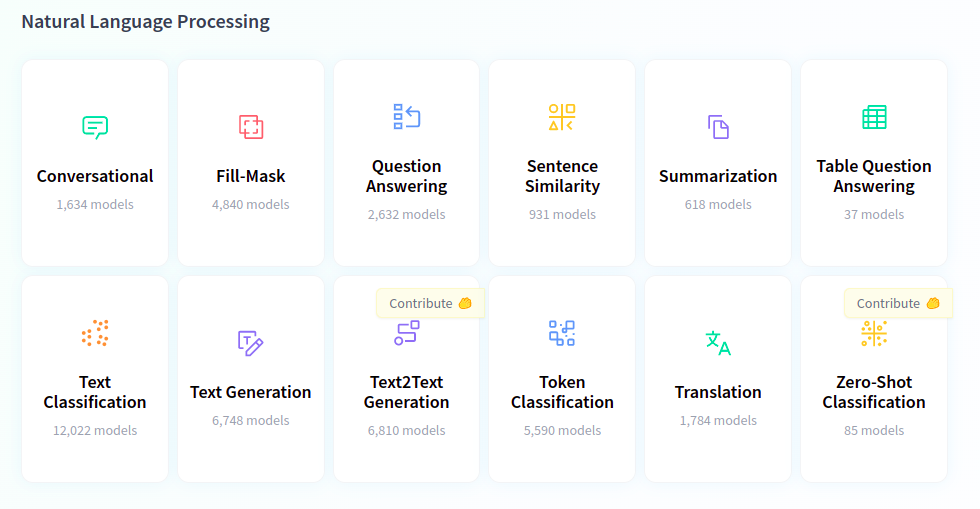
\includegraphics{images/hf-tasks.png}
\caption{tasks}
\end{figure}
\end{frame}

\begin{frame}[fragile]{Pipelines}
\protect\hypertarget{pipelines}{}
We can run many of these tasks, with any model we can find on
huggingface, with just a few lines of code using
\href{https://huggingface.co/docs/transformers/main_classes/pipelines}{Pipelines}.

\scriptsize

\begin{Shaded}
\begin{Highlighting}[]
\ImportTok{from}\NormalTok{ transformers }\ImportTok{import}\NormalTok{ pipeline}
\ImportTok{from}\NormalTok{ rich.pretty }\ImportTok{import}\NormalTok{ pprint}
\NormalTok{pipe }\OperatorTok{=}\NormalTok{ pipeline(}\StringTok{"sentiment{-}analysis"}\NormalTok{)}
\end{Highlighting}
\end{Shaded}

\begin{verbatim}
## No model was supplied, defaulted to distilbert-base-uncased-finetuned-sst-2-english and revision af0f99b (https://huggingface.co/distilbert-base-uncased-finetuned-sst-2-english).
## Using a pipeline without specifying a model name and revision in production is not recommended.
\end{verbatim}

\begin{Shaded}
\begin{Highlighting}[]
\NormalTok{res }\OperatorTok{=}\NormalTok{ pipe([}\StringTok{"This movie was really bad"}\NormalTok{, }\StringTok{"I loved watching this movie"}\NormalTok{])}
\NormalTok{pprint(res)}
\end{Highlighting}
\end{Shaded}

\begin{verbatim}
## [
## │   {'label': 'NEGATIVE', 'score': 0.9998040795326233},
## │   {'label': 'POSITIVE', 'score': 0.999700665473938}
## ]
\end{verbatim}
\end{frame}

\begin{frame}[fragile]{Pipelines - Text classification}
\protect\hypertarget{pipelines---text-classification}{}
If you look through the models on huggingface and
\href{https://huggingface.co/models?pipeline_tag=text-classification\&p=1\&sort=downloads}{filter
by task}, you will find a variety of pre-trained models for text
classification. Using one of these is simple.

\medskip
\scriptsize

\begin{Shaded}
\begin{Highlighting}[]
\NormalTok{pipe }\OperatorTok{=}\NormalTok{ pipeline(}\StringTok{"text{-}classification"}\NormalTok{, model}\OperatorTok{=}\StringTok{"nbroad/ESG{-}BERT"}\NormalTok{)}
\NormalTok{res }\OperatorTok{=}\NormalTok{ pipe(}\StringTok{"The Hertie School is committed to embedding and mainstreaming diversity, equity and inclusion into all areas of its activities."}\NormalTok{)}
\NormalTok{pprint(res)}
\end{Highlighting}
\end{Shaded}

\begin{verbatim}
## [
## │   {
## │   │   'label': 'Employee_Engagement_Inclusion_And_Diversity',
## │   │   'score': 0.9726636409759521
## │   }
## ]
\end{verbatim}
\end{frame}

\begin{frame}[fragile]{Pipelines - Text Generation (here be dragons!)}
\protect\hypertarget{pipelines---text-generation-here-be-dragons}{}
You can also use a model to generate text, but be warned this is likely
to cause convincing-sounding ``hallucinations''
\href{https://twitter.com/search?q=galactica\&src=typed_query}{examples
and discussion}.

\medskip
\scriptsize

\begin{Shaded}
\begin{Highlighting}[]
\ImportTok{from}\NormalTok{ textwrap }\ImportTok{import}\NormalTok{ wrap}
\NormalTok{run\_galactica }\OperatorTok{=} \VariableTok{False}
\ControlFlowTok{if}\NormalTok{ run\_galactica:}
\NormalTok{    pipe }\OperatorTok{=}\NormalTok{ pipeline(}\StringTok{"text{-}generation"}\NormalTok{, model}\OperatorTok{=}\StringTok{"facebook/galactica{-}1.3b"}\NormalTok{)}
\ControlFlowTok{else}\NormalTok{:}
\NormalTok{    pipe }\OperatorTok{=}\NormalTok{ pipeline(}\StringTok{"text{-}generation"}\NormalTok{)}
    
\end{Highlighting}
\end{Shaded}

\begin{verbatim}
## No model was supplied, defaulted to gpt2 and revision 6c0e608 (https://huggingface.co/gpt2).
## Using a pipeline without specifying a model name and revision in production is not recommended.
\end{verbatim}

\begin{Shaded}
\begin{Highlighting}[]
\NormalTok{res }\OperatorTok{=}\NormalTok{ pipe(}\StringTok{"Large language models can be useful. However,"}\NormalTok{)}
\end{Highlighting}
\end{Shaded}

\begin{verbatim}
## Setting `pad_token_id` to `eos_token_id`:50256 for open-end generation.
## /home/max/software/py39/lib/python3.9/site-packages/transformers/generation_utils.py:1202: UserWarning: Neither `max_length` nor `max_new_tokens` have been set, `max_length` will default to 50 (`self.config.max_length`). Controlling `max_length` via the config is deprecated and `max_length` will be removed from the config in v5 of Transformers -- we recommend using `max_new_tokens` to control the maximum length of the generation.
##   warnings.warn(
\end{verbatim}

\begin{Shaded}
\begin{Highlighting}[]
\NormalTok{pprint(wrap(res[}\DecValTok{0}\NormalTok{][}\StringTok{"generated\_text"}\NormalTok{]))}
\end{Highlighting}
\end{Shaded}

\begin{verbatim}
## [
## │   'Large language models can be useful. However, for small programs like',
## │   'Java, C++, C# or Objective-C, the language features of Java are a',
## │   'little off.  So, if you are looking for something a little different',
## │   'but not'
## ]
\end{verbatim}
\end{frame}

\begin{frame}{Exercise}
\protect\hypertarget{exercise}{}
Generate a response using any pipeline that shows the potential of
language models to cause \emph{harm}.

Describe a real world application in which it would do so.
\end{frame}

\begin{frame}[fragile]{Fine-tuning}
\protect\hypertarget{fine-tuning}{}
We can also fine-tune any pre-trained model for a classification problem
for which we have labelled examples. This requires a few steps, some not
inconsiderable computational power, and some patience.

Using GPUs speeds things up considerably.

We will run a small example on our own machines, with a small set of
texts.

\medskip

\scriptsize

\begin{Shaded}
\begin{Highlighting}[]
\CommentTok{\# Let\textquotesingle{}s take our texts and our labels again}
\NormalTok{texts, y }\OperatorTok{=} \BuiltInTok{zip}\NormalTok{(}
    \OperatorTok{*}\NormalTok{[}
\NormalTok{        (}\StringTok{"Climate change is impacting human systems"}\NormalTok{, }\DecValTok{1}\NormalTok{),}
\NormalTok{        (}\StringTok{"Climate change is caused by fossil fuels"}\NormalTok{, }\DecValTok{0}\NormalTok{),}
\NormalTok{        (}\StringTok{"Agricultural yields are affected by climate change"}\NormalTok{, }\DecValTok{1}\NormalTok{),}
\NormalTok{        (}\StringTok{"System change not climate change"}\NormalTok{, }\DecValTok{0}\NormalTok{),}
\NormalTok{        (}\StringTok{"higher temperatures are impacting human health"}\NormalTok{, }\DecValTok{1}\NormalTok{),}
\NormalTok{        (}\StringTok{"Forest fires are becoming more frequent due to climate change"}\NormalTok{, }\DecValTok{1}\NormalTok{),}
\NormalTok{        (}\StringTok{"Machine learning can read texts"}\NormalTok{, }\DecValTok{0}\NormalTok{),}
\NormalTok{        (}\StringTok{"AI can help solve climate change!"}\NormalTok{, }\DecValTok{0}\NormalTok{),}
\NormalTok{        (}\StringTok{"We need to save gas this winter"}\NormalTok{, }\DecValTok{0}\NormalTok{),}
\NormalTok{        (}\StringTok{"More frequent droughts are impacting crop yields"}\NormalTok{, }\DecValTok{1}\NormalTok{),}
\NormalTok{        (}\StringTok{"Many communities are affected by rising sea levels"}\NormalTok{, }\DecValTok{1}\NormalTok{),}
\NormalTok{        (}\StringTok{"Global emissions continue to rise"}\NormalTok{, }\DecValTok{0}\NormalTok{),}
\NormalTok{        (}\StringTok{"Ecosystems are increasingly impacted by rising temperatures"}\NormalTok{, }\DecValTok{1}\NormalTok{),}
\NormalTok{        (}\StringTok{"Emissions from fossil fuels need to decline"}\NormalTok{, }\DecValTok{0}\NormalTok{),}
\NormalTok{        (}\StringTok{"Anthropogenic climate change is impacting vulnerable communities"}\NormalTok{, }\DecValTok{1}\NormalTok{),}
\NormalTok{    ]}
\NormalTok{)}
\end{Highlighting}
\end{Shaded}
\end{frame}

\begin{frame}[fragile]{Tokenization}
\protect\hypertarget{tokenization}{}
First we need to tokenize our texts. It's easier if we put everything in
a huggingface dataset object and tokenize this

\medskip
\scriptsize

\begin{Shaded}
\begin{Highlighting}[]
\ImportTok{from}\NormalTok{ datasets }\ImportTok{import}\NormalTok{ Dataset}
\ImportTok{from}\NormalTok{ transformers }\ImportTok{import}\NormalTok{ AutoTokenizer}
\NormalTok{dataset }\OperatorTok{=}\NormalTok{ Dataset.from\_dict(\{}\StringTok{"text"}\NormalTok{: texts, }\StringTok{"label"}\NormalTok{: y\})}
\NormalTok{model\_name }\OperatorTok{=} \StringTok{"bert{-}base{-}uncased"}
\NormalTok{tokenizer }\OperatorTok{=}\NormalTok{ AutoTokenizer.from\_pretrained(model\_name)}
\KeywordTok{def}\NormalTok{ tokenize\_function(examples):}
    \ControlFlowTok{return}\NormalTok{ tokenizer(examples[}\StringTok{"text"}\NormalTok{], padding}\OperatorTok{=}\StringTok{"max\_length"}\NormalTok{, truncation}\OperatorTok{=}\VariableTok{True}\NormalTok{)}
\NormalTok{tokenized\_dataset }\OperatorTok{=}\NormalTok{ dataset.}\BuiltInTok{map}\NormalTok{(tokenize\_function, batched}\OperatorTok{=}\VariableTok{True}\NormalTok{)}
\end{Highlighting}
\end{Shaded}

\begin{verbatim}
##   0%|          | 0/1 [00:00<?, ?ba/s]100%|##########| 1/1 [00:00<00:00, 31.56ba/s]
\end{verbatim}

\begin{Shaded}
\begin{Highlighting}[]
\NormalTok{tokenized\_dataset}
\end{Highlighting}
\end{Shaded}

\begin{verbatim}
## Dataset({
##     features: ['text', 'label', 'input_ids', 'token_type_ids', 'attention_mask'],
##     num_rows: 15
## })
\end{verbatim}
\end{frame}

\begin{frame}[fragile]{Tokenization}
\protect\hypertarget{tokenization-1}{}
To make this even simpler, we can create a function that turns a list of
texts (and list of labels) into a tokenized dataset, given a tokenizer.

\medskip
\scriptsize

\begin{Shaded}
\begin{Highlighting}[]
\KeywordTok{def}\NormalTok{ datasetify(x, tokenizer, y}\OperatorTok{=}\VariableTok{None}\NormalTok{):}
\NormalTok{    data\_dict }\OperatorTok{=}\NormalTok{ \{}\StringTok{"text"}\NormalTok{: x\}}
    \ControlFlowTok{if}\NormalTok{ y }\KeywordTok{is} \KeywordTok{not} \VariableTok{None}\NormalTok{:}
\NormalTok{        data\_dict[}\StringTok{"label"}\NormalTok{] }\OperatorTok{=}\NormalTok{ y}
\NormalTok{    dataset }\OperatorTok{=}\NormalTok{ Dataset.from\_dict(data\_dict)}

    \KeywordTok{def}\NormalTok{ tokenize\_function(examples):}
        \ControlFlowTok{return}\NormalTok{ tokenizer(examples[}\StringTok{"text"}\NormalTok{], padding}\OperatorTok{=}\StringTok{"max\_length"}\NormalTok{, truncation}\OperatorTok{=}\VariableTok{True}\NormalTok{)}

    \ControlFlowTok{return}\NormalTok{ dataset.}\BuiltInTok{map}\NormalTok{(tokenize\_function, batched}\OperatorTok{=}\VariableTok{True}\NormalTok{)}
  
\NormalTok{train\_data }\OperatorTok{=}\NormalTok{ datasetify(texts, tokenizer, y)}
\end{Highlighting}
\end{Shaded}

\begin{verbatim}
##   0%|          | 0/1 [00:00<?, ?ba/s]100%|##########| 1/1 [00:00<00:00, 129.58ba/s]
\end{verbatim}
\end{frame}

\begin{frame}[fragile]{Training a model}
\protect\hypertarget{training-a-model}{}
We can load a model and train it using an instance of the
\texttt{Trainer} class.

\medskip
\scriptsize

\begin{Shaded}
\begin{Highlighting}[]
\ImportTok{from}\NormalTok{ transformers }\ImportTok{import}\NormalTok{ AutoModelForSequenceClassification, Trainer}
\CommentTok{\# We set num\_labels to 2 for binary classification, as we have two classes {-} positive and negative}
\NormalTok{model }\OperatorTok{=}\NormalTok{ AutoModelForSequenceClassification.from\_pretrained(model\_name, num\_labels}\OperatorTok{=}\DecValTok{2}\NormalTok{)}
\end{Highlighting}
\end{Shaded}

\begin{verbatim}
## Some weights of the model checkpoint at bert-base-uncased were not used when initializing BertForSequenceClassification: ['cls.predictions.bias', 'cls.predictions.decoder.weight', 'cls.seq_relationship.bias', 'cls.seq_relationship.weight', 'cls.predictions.transform.dense.weight', 'cls.predictions.transform.LayerNorm.weight', 'cls.predictions.transform.dense.bias', 'cls.predictions.transform.LayerNorm.bias']
## - This IS expected if you are initializing BertForSequenceClassification from the checkpoint of a model trained on another task or with another architecture (e.g. initializing a BertForSequenceClassification model from a BertForPreTraining model).
## - This IS NOT expected if you are initializing BertForSequenceClassification from the checkpoint of a model that you expect to be exactly identical (initializing a BertForSequenceClassification model from a BertForSequenceClassification model).
## Some weights of BertForSequenceClassification were not initialized from the model checkpoint at bert-base-uncased and are newly initialized: ['classifier.bias', 'classifier.weight']
## You should probably TRAIN this model on a down-stream task to be able to use it for predictions and inference.
\end{verbatim}

\begin{Shaded}
\begin{Highlighting}[]
\NormalTok{trainer }\OperatorTok{=}\NormalTok{ Trainer(model}\OperatorTok{=}\NormalTok{model, train\_dataset}\OperatorTok{=}\NormalTok{datasetify(texts, tokenizer, y))}
\CommentTok{\# Once this has been instantiated we can apply the train() method}
\end{Highlighting}
\end{Shaded}

\begin{verbatim}
##   0%|          | 0/1 [00:00<?, ?ba/s]100%|##########| 1/1 [00:00<00:00, 158.56ba/s]
\end{verbatim}

\begin{Shaded}
\begin{Highlighting}[]
\NormalTok{trainer.train()}
\end{Highlighting}
\end{Shaded}

\begin{verbatim}
## {'train_runtime': 5870.6374, 'train_samples_per_second': 0.008, 'train_steps_per_second': 0.001, 'train_loss': 0.6716297467549642, 'epoch': 3.0}
## TrainOutput(global_step=6, training_loss=0.6716297467549642, metrics={'train_runtime': 5870.6374, 'train_samples_per_second': 0.008, 'train_steps_per_second': 0.001, 'train_loss': 0.6716297467549642, 'epoch': 3.0})
## 
## The following columns in the training set don't have a corresponding argument in `BertForSequenceClassification.forward` and have been ignored: text. If text are not expected by `BertForSequenceClassification.forward`,  you can safely ignore this message.
## /home/max/software/py39/lib/python3.9/site-packages/transformers/optimization.py:306: FutureWarning: This implementation of AdamW is deprecated and will be removed in a future version. Use the PyTorch implementation torch.optim.AdamW instead, or set `no_deprecation_warning=True` to disable this warning
##   warnings.warn(
## ***** Running training *****
##   Num examples = 15
##   Num Epochs = 3
##   Instantaneous batch size per device = 8
##   Total train batch size (w. parallel, distributed & accumulation) = 8
##   Gradient Accumulation steps = 1
##   Total optimization steps = 6
##   0%|          | 0/6 [00:00<?, ?it/s] 17%|#6        | 1/6 [02:31<12:38, 151.64s/it] 33%|###3      | 2/6 [04:07<07:54, 118.64s/it] 50%|#####     | 3/6 [1:33:48<2:06:05, 2521.67s/it] 67%|######6   | 4/6 [1:35:05<51:53, 1556.66s/it]   83%|########3 | 5/6 [1:36:33<17:07, 1027.07s/it]100%|##########| 6/6 [1:37:50<00:00, 703.98s/it] 
## 
## Training completed. Do not forget to share your model on huggingface.co/models =)
## 
## 
##                                                 100%|##########| 6/6 [1:37:50<00:00, 703.98s/it]100%|##########| 6/6 [1:37:50<00:00, 978.44s/it]
\end{verbatim}
\end{frame}

\begin{frame}[fragile]{Making predictions}
\protect\hypertarget{making-predictions}{}
With a trained model, we can make predictions on a set of new texts

\medskip
\scriptsize

\begin{Shaded}
\begin{Highlighting}[]
\CommentTok{\# To generate predictions, we just need to supply a dataset to the predict method}
\NormalTok{new\_texts }\OperatorTok{=}\NormalTok{ [}
    \StringTok{"climate change is impacting terrestrial ecosystems"}\NormalTok{,}
    \StringTok{"Machine Learning will solve climate change"}\NormalTok{,}
    \StringTok{"Fossil fuels are responsible for rising temperature"}\NormalTok{,}
\NormalTok{]}
\NormalTok{new\_y }\OperatorTok{=}\NormalTok{ [}\DecValTok{1}\NormalTok{,}\DecValTok{0}\NormalTok{,}\DecValTok{0}\NormalTok{]}

\NormalTok{pred }\OperatorTok{=}\NormalTok{ trainer.predict(datasetify(new\_texts, tokenizer, new\_y))}
\end{Highlighting}
\end{Shaded}

\begin{verbatim}
##   0%|          | 0/1 [00:00<?, ?ba/s]100%|##########| 1/1 [00:00<00:00, 36.82ba/s]
## The following columns in the test set don't have a corresponding argument in `BertForSequenceClassification.forward` and have been ignored: text. If text are not expected by `BertForSequenceClassification.forward`,  you can safely ignore this message.
## ***** Running Prediction *****
##   Num examples = 3
##   Batch size = 8
##   0%|          | 0/1 [00:00<?, ?it/s]100%|##########| 1/1 [00:00<00:00, 1332.79it/s]
\end{verbatim}

\begin{Shaded}
\begin{Highlighting}[]
\NormalTok{pred}
\end{Highlighting}
\end{Shaded}

\begin{verbatim}
## PredictionOutput(predictions=array([[-0.44623327,  0.07649825],
##        [-0.04447261,  0.04163995],
##        [-0.1721632 ,  0.10295288]], dtype=float32), label_ids=array([1, 0, 0]), metrics={'test_loss': 0.6809406876564026, 'test_runtime': 10.9274, 'test_samples_per_second': 0.275, 'test_steps_per_second': 0.092})
\end{verbatim}
\end{frame}

\begin{frame}[fragile]{Turning logits into probabilities}
\protect\hypertarget{turning-logits-into-probabilities}{}
As we did last week, we need a variation of the \textbf{sigmoid}
function (\textbf{Softmax}) to turn our predictions (which are returned
as logits) into probabilities. The softmax activation function ensures
the probabilities for each class add up to 1 for each document. Note
that these probabilities are not necessarily well calibrated.

\medskip
\scriptsize

\begin{Shaded}
\begin{Highlighting}[]
\CommentTok{\# To generate predictions, we just need to supply a dataset to the predict method}
\ImportTok{from}\NormalTok{ torch }\ImportTok{import}\NormalTok{ tensor}
\ImportTok{from}\NormalTok{ torch.nn }\ImportTok{import}\NormalTok{ Sigmoid, Softmax}
\NormalTok{activation }\OperatorTok{=}\NormalTok{ (Softmax())}
\NormalTok{activation(tensor(pred.predictions))}
\end{Highlighting}
\end{Shaded}

\begin{verbatim}
## tensor([[0.3722, 0.6278],
##         [0.4785, 0.5215],
##         [0.4317, 0.5683]])
## 
## <string>:1: UserWarning: Implicit dimension choice for softmax has been deprecated. Change the call to include dim=X as an argument.
\end{verbatim}
\end{frame}

\begin{frame}[fragile]{Creating a predict\_proba function}
\protect\hypertarget{creating-a-predict_proba-function}{}
If we miss our predict\_proba function from sklearn, we can
\emph{subclass} Trainer, to provide an additional method

\medskip
\scriptsize

\begin{Shaded}
\begin{Highlighting}[]
\ImportTok{from}\NormalTok{ transformers.trainer\_utils }\ImportTok{import}\NormalTok{ PredictionOutput}

\KeywordTok{class}\NormalTok{ ProbTrainer(Trainer):}
    \KeywordTok{def}\NormalTok{ predict\_proba(}\VariableTok{self}\NormalTok{, test\_dataset: Dataset) }\OperatorTok{{-}\textgreater{}}\NormalTok{ PredictionOutput:}
\NormalTok{        logits }\OperatorTok{=} \VariableTok{self}\NormalTok{.predict(test\_dataset).predictions}
\NormalTok{        activation }\OperatorTok{=}\NormalTok{ Softmax()}
        \ControlFlowTok{return}\NormalTok{ activation(tensor(logits)).numpy()}


\NormalTok{trainer }\OperatorTok{=}\NormalTok{ ProbTrainer(model}\OperatorTok{=}\NormalTok{model, train\_dataset}\OperatorTok{=}\NormalTok{datasetify(texts, tokenizer, y))}
\end{Highlighting}
\end{Shaded}

\begin{verbatim}
##   0%|          | 0/1 [00:00<?, ?ba/s]100%|##########| 1/1 [00:00<00:00, 228.55ba/s]
## No `TrainingArguments` passed, using `output_dir=tmp_trainer`.
## PyTorch: setting up devices
## The default value for the training argument `--report_to` will change in v5 (from all installed integrations to none). In v5, you will need to use `--report_to all` to get the same behavior as now. You should start updating your code and make this info disappear :-).
\end{verbatim}

\begin{Shaded}
\begin{Highlighting}[]
\NormalTok{trainer.train()}
\end{Highlighting}
\end{Shaded}

\begin{verbatim}
## {'train_runtime': 22.1918, 'train_samples_per_second': 2.028, 'train_steps_per_second': 0.27, 'train_loss': 0.30997474988301593, 'epoch': 3.0}
## TrainOutput(global_step=6, training_loss=0.30997474988301593, metrics={'train_runtime': 22.1918, 'train_samples_per_second': 2.028, 'train_steps_per_second': 0.27, 'train_loss': 0.30997474988301593, 'epoch': 3.0})
## 
## The following columns in the training set don't have a corresponding argument in `BertForSequenceClassification.forward` and have been ignored: text. If text are not expected by `BertForSequenceClassification.forward`,  you can safely ignore this message.
## ***** Running training *****
##   Num examples = 15
##   Num Epochs = 3
##   Instantaneous batch size per device = 8
##   Total train batch size (w. parallel, distributed & accumulation) = 8
##   Gradient Accumulation steps = 1
##   Total optimization steps = 6
##   0%|          | 0/6 [00:00<?, ?it/s] 17%|#6        | 1/6 [00:03<00:16,  3.35s/it] 33%|###3      | 2/6 [00:07<00:14,  3.73s/it] 50%|#####     | 3/6 [00:10<00:10,  3.59s/it] 67%|######6   | 4/6 [00:14<00:07,  3.74s/it] 83%|########3 | 5/6 [00:18<00:03,  3.64s/it]100%|##########| 6/6 [00:22<00:00,  3.74s/it]
## 
## Training completed. Do not forget to share your model on huggingface.co/models =)
## 
## 
##                                              100%|##########| 6/6 [00:22<00:00,  3.74s/it]100%|##########| 6/6 [00:22<00:00,  3.69s/it]
\end{verbatim}
\end{frame}

\begin{frame}[fragile]{Creating a predict\_proba function}
\protect\hypertarget{creating-a-predict_proba-function-1}{}
If we miss our predict\_proba function from sklearn, we can
\emph{subclass} Trainer, to provide an additional method

\medskip
\scriptsize

\begin{Shaded}
\begin{Highlighting}[]
\NormalTok{pred }\OperatorTok{=}\NormalTok{ trainer.predict\_proba(datasetify(new\_texts, tokenizer))}
\end{Highlighting}
\end{Shaded}

\begin{verbatim}
##   0%|          | 0/1 [00:00<?, ?ba/s]100%|##########| 1/1 [00:00<00:00, 294.83ba/s]
## The following columns in the test set don't have a corresponding argument in `BertForSequenceClassification.forward` and have been ignored: text. If text are not expected by `BertForSequenceClassification.forward`,  you can safely ignore this message.
## ***** Running Prediction *****
##   Num examples = 3
##   Batch size = 8
##   0%|          | 0/1 [00:00<?, ?it/s]100%|##########| 1/1 [00:00<00:00, 3339.41it/s]
## <string>:5: UserWarning: Implicit dimension choice for softmax has been deprecated. Change the call to include dim=X as an argument.
\end{verbatim}

\begin{Shaded}
\begin{Highlighting}[]
\NormalTok{pred}
\end{Highlighting}
\end{Shaded}

\begin{verbatim}
## array([[0.2340269 , 0.7659731 ],
##        [0.7636742 , 0.23632582],
##        [0.84745055, 0.15254942]], dtype=float32)
\end{verbatim}
\end{frame}

\begin{frame}[fragile]{Hyperparameters}
\protect\hypertarget{hyperparameters}{}
The original BERT paper defined a hyperparameter space that should be
searched when fine-tuning a BERT model. These are data-dependent and
values outside these ranges may make improvements in some contexts.

\medskip
\scriptsize

\begin{Shaded}
\begin{Highlighting}[]
\NormalTok{params }\OperatorTok{=}\NormalTok{ \{}
  \StringTok{"batch\_size"}\NormalTok{: [}\DecValTok{16}\NormalTok{, }\DecValTok{32}\NormalTok{],}
  \StringTok{"learning\_rate"}\NormalTok{: [}\FloatTok{5e{-}5}\NormalTok{, }\FloatTok{3e{-}5}\NormalTok{, }\FloatTok{2e{-}5}\NormalTok{],}
  \StringTok{"number of epochs"}\NormalTok{: [}\DecValTok{2}\NormalTok{,}\DecValTok{3}\NormalTok{,}\DecValTok{4}\NormalTok{]}
\NormalTok{\}}
\ImportTok{import}\NormalTok{ itertools}
\KeywordTok{def}\NormalTok{ product\_dict(}\OperatorTok{**}\NormalTok{kwargs):}
\NormalTok{    keys }\OperatorTok{=}\NormalTok{ kwargs.keys()}
\NormalTok{    vals }\OperatorTok{=}\NormalTok{ kwargs.values()}
    \ControlFlowTok{for}\NormalTok{ instance }\KeywordTok{in}\NormalTok{ itertools.product(}\OperatorTok{*}\NormalTok{vals):}
        \ControlFlowTok{yield} \BuiltInTok{dict}\NormalTok{(}\BuiltInTok{zip}\NormalTok{(keys, instance))}
\NormalTok{param\_space }\OperatorTok{=} \BuiltInTok{list}\NormalTok{(product\_dict(}\OperatorTok{**}\NormalTok{params))}
\BuiltInTok{len}\NormalTok{(param\_space)}
\end{Highlighting}
\end{Shaded}

\begin{verbatim}
## 18
\end{verbatim}
\end{frame}

\begin{frame}[fragile]{Hyperparameters}
\protect\hypertarget{hyperparameters-1}{}
We can plug these values into a TrainingArguments object, which we pass
to our trainer. This would take quite some time.

\medskip
\scriptsize

\begin{Shaded}
\begin{Highlighting}[]
\ImportTok{from}\NormalTok{ transformers }\ImportTok{import}\NormalTok{ TrainingArguments}
\ControlFlowTok{for}\NormalTok{ p }\KeywordTok{in}\NormalTok{ param\_space:}
\NormalTok{    training\_args }\OperatorTok{=}\NormalTok{ TrainingArguments(}
\NormalTok{        num\_train\_epochs}\OperatorTok{=}\NormalTok{p[}\StringTok{"number of epochs"}\NormalTok{],}
\NormalTok{        learning\_rate}\OperatorTok{=}\NormalTok{p[}\StringTok{"learning\_rate"}\NormalTok{],}
\NormalTok{        per\_device\_train\_batch\_size}\OperatorTok{=}\NormalTok{p[}\StringTok{"batch\_size"}\NormalTok{],}
\NormalTok{        output\_dir}\OperatorTok{=}\StringTok{"out"}
\NormalTok{    )}
\NormalTok{    trainer }\OperatorTok{=}\NormalTok{ ProbTrainer(model}\OperatorTok{=}\NormalTok{model, train\_dataset}\OperatorTok{=}\NormalTok{datasetify(texts, tokenizer, y), args}\OperatorTok{=}\NormalTok{training\_args)}
\NormalTok{    trainer.train()}
    \CommentTok{\# Evaluate our model}
\end{Highlighting}
\end{Shaded}
\end{frame}

\begin{frame}{Pre-training}
\protect\hypertarget{pre-training}{}
If we have lots of \emph{unlabelled} data from a specific domain, doing
additional \emph{pretraining} of a transformer-based model may increase
its performance in classifying \emph{labelled} data.

See \href{https://aclanthology.org/2020.acl-main.740/}{Don't Stop
Pretraining: Adapt Language Models to Domains and Tasks}.

However, this is \emph{much} more resource intensive, and there are now
thousands of models available, some of which might have been trained on
similar data.
\end{frame}

\begin{frame}{Exercise - Training your own model}
\protect\hypertarget{exercise---training-your-own-model}{}
In small groups, repeat the classification task in last week's slides
with a model of your choosing from transformers.

Did the model perform better or worse than our support vector machine?
\end{frame}

\hypertarget{spacy}{%
\section{Spacy}\label{spacy}}

\begin{frame}{What is spacy}
\protect\hypertarget{what-is-spacy}{}
Spacy provides ``industrial-strength'' Natural Language Processing.

It is most useful for processing texts, but its latest version also
claims support for Transformers and the huggingface model ecosystem.

We'll explore a few examples to get you used to the syntax and
documentation
\end{frame}

\begin{frame}[fragile]{Advanced tokenization}
\protect\hypertarget{advanced-tokenization}{}
You can process a document into a list of tokens with Spacy, and each
token contains many \href{https://spacy.io/api/token}{attributes and
methods}

\medskip
\scriptsize

\begin{Shaded}
\begin{Highlighting}[]
\ImportTok{import}\NormalTok{ spacy}
\NormalTok{nlp }\OperatorTok{=}\NormalTok{ spacy.load(}\StringTok{"en\_core\_web\_md"}\NormalTok{)}
\NormalTok{text }\OperatorTok{=} \StringTok{"Students at the Hertie School in Berlin learn how to use Spacy"}
\NormalTok{doc }\OperatorTok{=}\NormalTok{ nlp(text)}
\ControlFlowTok{for}\NormalTok{ token }\KeywordTok{in}\NormalTok{ doc:}
    \BuiltInTok{print}\NormalTok{(token.text, token.lemma\_, token.pos\_,token.is\_stop)}
\end{Highlighting}
\end{Shaded}

\begin{verbatim}
## Students student NOUN False
## at at ADP True
## the the DET True
## Hertie Hertie PROPN False
## School School PROPN False
## in in ADP True
## Berlin Berlin PROPN False
## learn learn VERB False
## how how SCONJ True
## to to PART True
## use use VERB False
## Spacy Spacy PROPN False
\end{verbatim}
\end{frame}

\begin{frame}[fragile]{Named Entity Recognition}
\protect\hypertarget{named-entity-recognition}{}
Named entities are real-world objects referred to in a text. Spacy can
guess what phrases are what types of real-word objects.

\medskip
\scriptsize

\begin{Shaded}
\begin{Highlighting}[]
\NormalTok{nlp }\OperatorTok{=}\NormalTok{ spacy.load(}\StringTok{"en\_core\_web\_md"}\NormalTok{)}
\NormalTok{doc }\OperatorTok{=}\NormalTok{ nlp(text)}
\ControlFlowTok{for}\NormalTok{ ent }\KeywordTok{in}\NormalTok{ doc.ents:}
    \BuiltInTok{print}\NormalTok{(ent.text, ent.label\_)}
\end{Highlighting}
\end{Shaded}

\begin{verbatim}
## the Hertie School ORG
## Berlin GPE
\end{verbatim}
\end{frame}

\begin{frame}[fragile]{Embeddings in Spacy}
\protect\hypertarget{embeddings-in-spacy}{}
Spacy also already puts our documents and tokens into an embedding space

\medskip
\scriptsize

\begin{Shaded}
\begin{Highlighting}[]
\NormalTok{nlp }\OperatorTok{=}\NormalTok{ spacy.load(}\StringTok{"en\_core\_web\_md"}\NormalTok{)}
\NormalTok{doc }\OperatorTok{=}\NormalTok{ nlp(text)}
\NormalTok{tok }\OperatorTok{=}\NormalTok{ doc[}\DecValTok{0}\NormalTok{]}
\BuiltInTok{print}\NormalTok{(tok.vector.shape)}
\end{Highlighting}
\end{Shaded}

\begin{verbatim}
## (300,)
\end{verbatim}

\begin{Shaded}
\begin{Highlighting}[]
\NormalTok{texts }\OperatorTok{=}\NormalTok{ [}
  \StringTok{"The acclaimed author penned novels based on her life"}\NormalTok{,}
  \StringTok{"Nobel prize{-}winning writer writes autobiographical fiction"}
\NormalTok{]}
\NormalTok{docs }\OperatorTok{=}\NormalTok{ [nlp(t) }\ControlFlowTok{for}\NormalTok{ t }\KeywordTok{in}\NormalTok{ texts]}
\NormalTok{docs[}\DecValTok{0}\NormalTok{].similarity(docs[}\DecValTok{1}\NormalTok{])}
\end{Highlighting}
\end{Shaded}

\begin{verbatim}
## 0.6186866838865561
\end{verbatim}
\end{frame}

\begin{frame}{Exercise}
\protect\hypertarget{exercise-1}{}
In small groups, retrieve our manifesto dataset.

Extract only the adjectives from the manifestos.

Which adjectives are used most often by each party?
\end{frame}

\hypertarget{wrapup}{%
\section{Wrapup}\label{wrapup}}

\begin{frame}{Wrapup}
\protect\hypertarget{wrapup-1}{}
Today we have covered

\begin{itemize}
\tightlist
\item
  How transformer-based models work (at a very high level) and what they
  do
\item
  How to use pre-trained models for a variety of tasks
\item
  How to fine-tune existing models for our own classification tasks
\item
  How to use spacy
\end{itemize}

This concludes the input part of the course!
\end{frame}

\begin{frame}{Assignment 3}
\protect\hypertarget{assignment-3}{}
Next week we'll see 7 student presentations.

Each group will have \textbf{8} minutes to present (\emph{strictly
enforced}), with 4 minutes for questions (mainly from the audience!).

Present directly from your laptop, which we will connect to the
projector via HDMI cable (bring an adaptor if necessary). Try to keep
transitions \textless{} 1 minute!
\end{frame}

\begin{frame}[allowframebreaks]{}
  \bibliographytrue
  \bibliography{../presentation-resources/MyLibrary.bib}
\end{frame}

\end{document}
